%%%%%%%%%%%%%%%%%%%%%%%%%%%%%%%%%%%%%%%%%
% Thin Sectioned Essay
% LaTeX Template
% Version 1.0 (3/8/13)
%
% This template has been downloaded from:
% http://www.LaTeXTemplates.com
%
% Original Author:
% Nicolas Diaz (nsdiaz@uc.cl) with extensive modifications by:
% Vel (vel@latextemplates.com)
%
% License:
% CC BY-NC-SA 3.0 (http://creativecommons.org/licenses/by-nc-sa/3.0/)
%
%%%%%%%%%%%%%%%%%%%%%%%%%%%%%%%%%%%%%%%%%

%----------------------------------------------------------------------------------------
%   PACKAGES AND OTHER DOCUMENT CONFIGURATIONS
%----------------------------------------------------------------------------------------

\documentclass[11pt]{article} % Font size (can be 10pt, 11pt or 12pt) and paper size (remove a4paper for US letter paper)

\usepackage[utf8]{inputenc} % Set utf8 code
\usepackage[protrusion=true,expansion=true]{microtype} % Better typography
\usepackage[portuguese]{babel}
\usepackage{graphicx} % Required for including pictures
\usepackage{wrapfig} % Allows in-line images
\usepackage[pagebackref]{hyperref}

\usepackage{mathpazo} % Use the Palatino font
\usepackage[T1]{fontenc} % Required for accented characters

\usepackage{wallpaper}
\usepackage[font={color=white,bf},figurename=Fig.,labelfont={it}]{caption}
\usepackage{lipsum, xcolor, etoolbox, footmisc, bigfoot}

\usepackage{tabu}
\hypersetup{
    colorlinks=false,
    pdfborder={0 0 0},
}

\setcounter{secnumdepth}{5}
\setcounter{tocdepth}{5}

\linespread{1.05} % Change line spacing here, Palatino benefits from a slight increase by default

\makeatletter
\renewcommand\@biblabel[1]{\textbf{#1.}} % Change the square brackets for each bibliography item from '[1]' to '1.'
\renewcommand{\@listI}{\itemsep=0pt} % Reduce the space between items in the itemize and enumerate environments and the bibliography

\renewcommand{\maketitle}{ % Customize the title - do not edit title and author name here, see the TITLE block below


\begin{center} % Right align
{\LARGE\@title} % Increase the font size of the title

\vspace{20pt} % Some vertical space between the title and author name

\end{center}
}

\patchcmd{\ps@plain}{\thepage}{\textcolor{white}{\thepage}}{}{}
\makeatother

\begin{document}

\ThisTileWallPaper{\paperwidth}{\paperheight}{res/wallpaper_header.jpg}
\color{white}
\pagestyle{plain}
\def\footnotelayout{\color{white}}
\renewcommand\thefootnote{\textcolor{white}{\arabic{footnote}}}
\begin{titlepage}
 \vfill
  \begin{center}
   {\textbf{{{\Huge  Strife Of Mythology Tower Defense}}}}\\[6cm]


   {{\huge Game Design Document}}\\[6cm]

   \hspace{.45\textwidth} %posiciona a minipage
  \vfill

\vspace{2cm}

\large \textbf{Brasília}

\large \textbf{Abril de 2016}
\end{center}
\end{titlepage}
\newpage
\color{black}
\tableofcontents

\newpage

%----------------------------------------------------------------------------------------
%   DOC BODY
%----------------------------------------------------------------------------------------

\TileWallPaper{\paperwidth}{\paperheight}{res/wallpaper_body.jpg}
\color{white}

\section*{Tabela de Revisão}


\begin{table}[h]

  \taburulecolor{white}
  \color{white}
\begin{tabu}{|l|l|p{60mm}|l|}

\hline 
\textbf{Versão}     & \textbf{Data}     & \textbf{Descrição}                              			& \textbf{Autor}    \\ \hline
0.1                 & 05/03/16        & Objetivo / História / Controles                    			& Marcelo Martins     \\ \hline
0.2                 & 06/03/16        & Requisitos Tecnológicos                            			& Marcelo Martins     \\ \hline
0.3                 & 13/03/16        & Aplicando correções propostas                      			& Marcelo Martins     \\ \hline
0.4                 & 12/04/16      & Adição dos Personagens / Refinamento dos itens anteriores   	& Marcelo Martins     \\ \hline
0.5                 & 29/04/2015        & Rascunho das telas				                   			& Jônntas Lennon     \\ \hline
0.6                 & 10/05/2015        & telas / Personagens				                   			& Jônntas Lennon     \\ \hline
0.7                 & 18/05/2015        & Economia				                   			& Jônntas e Marcelo     \\ \hline
0.8                 & 18/05/2015        & Personagens				                   			& Jônntas e Marcelo     \\ \hline


\end{tabu}
\end{table}

\newpage

\section{Objetivo do jogo}

O \textit{\textbf{SoMTD}} é um jogo de estilo\textit{ Tower Defense}, onde o objetivo é impedir que as \textit{waves} de monstros avancem pela caminho utilizando torres que atacam estas \textit{waves}, estas torres são pertencentes a três Deuses.
 A medida em que as \textit{waves} são vencidas, elas ficam mais fortes e difíceis de derrotar. Nisto haverá um recurso que servirá para evoluir e construir novas torres, o qual será obtido conforme os monstros forem derrotados.

\section{Glossário}
\begin{itemize}
\item \textbf{Wave}: Inimigos que nascem em conjunto em momentos do jogo.
\item \textbf{Caminho}: Caminho pré-determinado que será seguido pelas \textit{waves}. Caso um inimigo chegue ao fim da trilha, o jogador sofre uma punição.
\item \textbf{Tower Defense}: Um estilo de jogo onde um jogador deve impedir unidades inimigas de completarem seu objetivo utilizando torres.
\item \textbf{Health Point(HP)}: Atributo referente a vida \textit{player}.
\item \textbf{Def} - Defense : refere-se neste contexto, aos pontos de ataques ao monstro, a defesa aqui é o nível de resistência a ataques comuns.
\item \textbf{Sp} - Speed : refere-se a velocidade com que as waves se movem.
\item \textbf{gold}: única remuneração do jogo.
\end{itemize} 
 
\section{Conceito do jogo}

As torres pertencem  três Deuses sendo eles:
\begin{itemize}
\item Hades.
\item Zeus.
\item Poseidom.
\end{itemize}

Cada Deus terá um conjunto de Torres a seu dispor, divididas em 2 categorias sendo que cada categoria possuirá uma singularidade em relação as demais, possuindo assim vantagens em relação a alguns tipos de monstros e desvantagens em relação a outros tipos de monstros.

Ao iniciar o jogo, o jogador terá uma quantidade de ouro suficiente para adquirir e colocar torres de forma estratégica, tentando evitar a passagem dos inimigos pela trilha, sendo que no início do jogo apenas um tipo de torre por Deus estará disponível, tais torres podem ser evoluídas ao passo que a torre selecionada consiga destruir os monstros. 

A mudança de cenário ocorrerá ao decorrer do jogo, a medida em que as \textit{waves} forem derrotadas o jogador alcançará pontos de performance, que ao completar a barra referente a estes pontos, ocorrerá uma troca de era, havendo assim a mudança de fase e consequentemente de cenário. 

O final do jogo pode-se dar de duas formas:

\begin{enumerate}
\item O jogador posicionou as torres da forma que ele acreditava ser a forma mais estratégica, contudo não era a melhor forma, e ele não conseguiu suportar a \textit{wave},fazendo com que os inimigos cheguem ao final da trilha, com isso ele irá acumular penalidades, atingindo o máximo de penalidades aparecera a mensagem de \textit{Game Over};
\item O jogador consegue posicionar as torres da forma mais estratégica, conseguindo assim, suportar todas as \textit{waves} impostas, caso isso ocorra, ele irá receber uma mensagem de \textit{You Win}.

\end{enumerate}

\section{Gameplay}

\subsection{Progressão do Jogo}

\subsection{Timer}

\newpage

\section{Mecânicas do Jogo}
\subsubsection{Movimentação}
A movimentação das waves será em um caminho pré-determinado, cabendo ao jogador apenas posicionar as torres com o mouse próxima a esse caminho, não havendo assim movimentação por parte do jogador principal.

\subsubsection{Resolução}
\newpage

\subsection{Recursos}

O jogo contará com 3 recursos distintos para realizar a progressão da base e dos personagens, sendo eles Data, Matéria e Energia.

\subsection{Estrutura}

\newpage

\section{Câmera e HUD}

\subsection{Câmera}

A câmera do jogo será 2D estática em um mapa isométrico, como exemplificado pela imagem abaixo.
\begin{figure}[!htp]
\centering
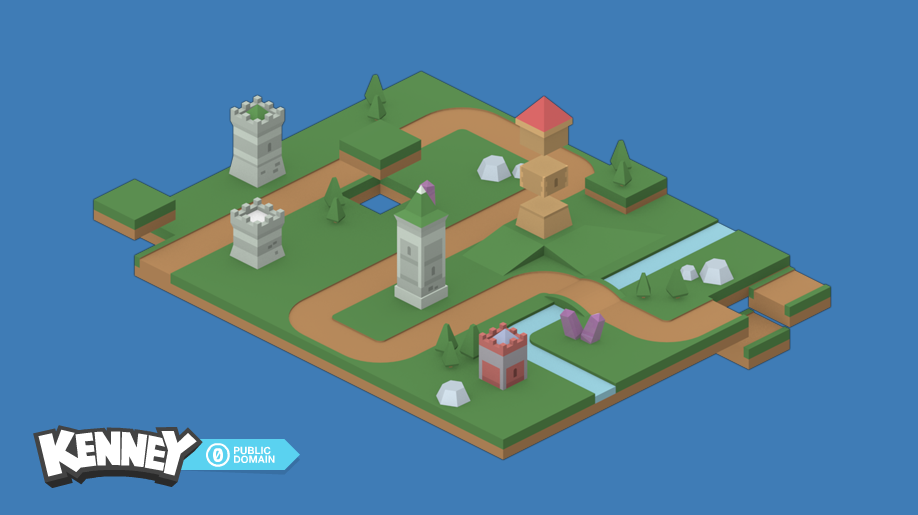
\includegraphics[scale=0.25]{res/map_example.png}
\caption{Tela Câmera}
\label{Tela Barracks}
\end{figure}

\subsection{HUD}

O HUD (Heads-Up Display) será composto de um menu inferior o qual será dividido em três secções, sendo elas:
\begin{itemize}
\item Um circulo contendo o Deus selecionado, ao clicar neste Deus, automaticamente ocorrerá a troca para o próximo Deus.
\item A direita do circulo tem-se uma barra de HP, que decairá quando as \textit{waves} atravessarem o caminho, além das informações de gold disponíveis para incrementar as torres.
\item Finalizando tem-se as informações referentes aos \textit{Tiers} das torres, associadas aos Deuses.
\end{itemize}

\begin{figure}[!htp]
\centering
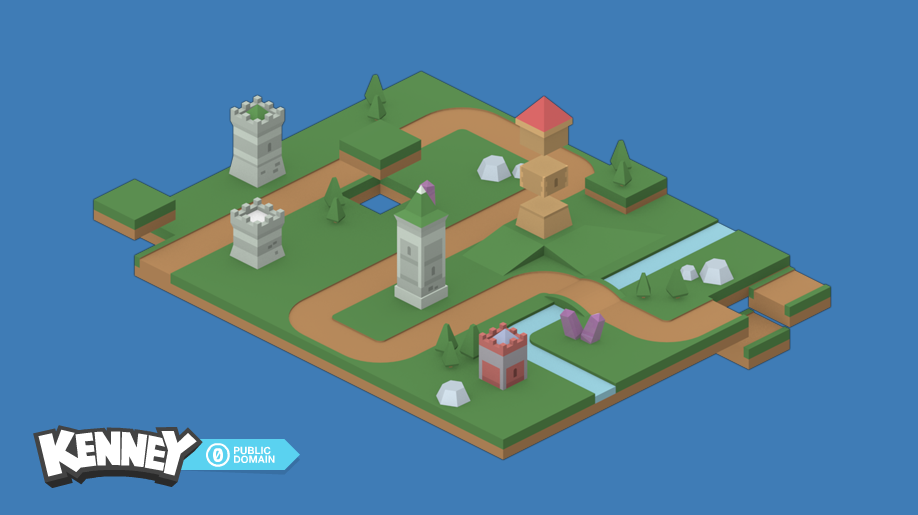
\includegraphics[scale=0.25]{res/map_example.png}
\caption{Hud}
\label{HUD}
\end{figure}

Na tela \textit{é apresentado} todos os equipamentos no qual o personagem poderá utilizar durante o combate que se passarão durante a exploração vertical.

\begin{figure}[!htp]
\centering
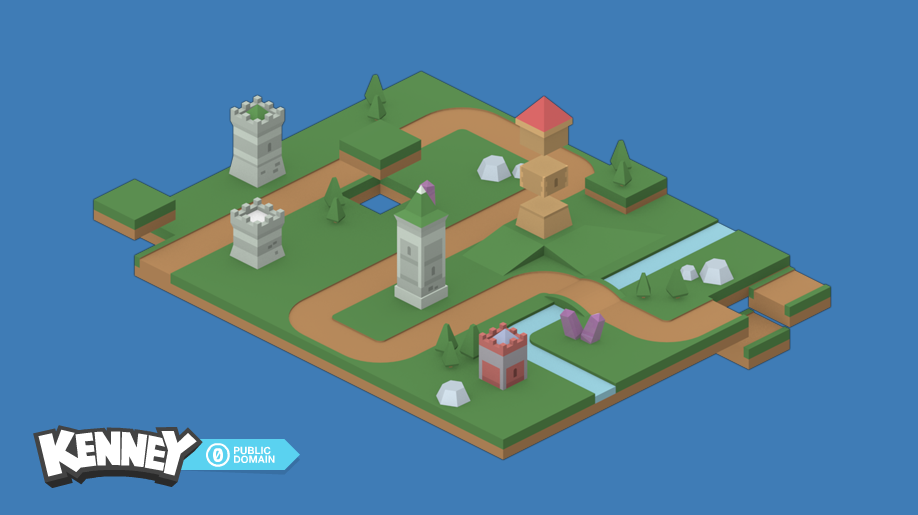
\includegraphics[scale=0.25]{res/map_example.png}
\caption{Tela Equip}
\label{Tela Equip}
\end{figure}

\newpage

\section{Personagens Principais}

\subsection{Deuses}
Como dito nas secções anteriores, haverão 3 Deuses:

{\large \textbf{Zeus}}:, sendo um Deus, cujo as torres utilizam predominantemente raios para atacar, possuirá dano maior em inimigos do tipo fly.
\begin{figure}[!htp]
\centering
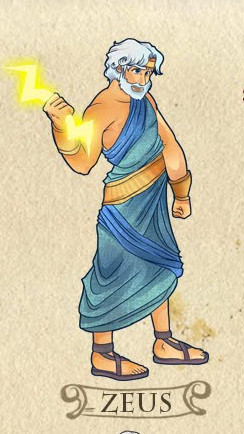
\includegraphics[scale=0.25]{res/characters/zeus.png}
\caption{Exemplo de Zeus}
\label{zeus}
\end{figure}

{\large \textbf{Poseidon}}: suas torres utilizam o poder das águas para atacar, possuirá dano maior em  inimigos do tipo speed.
\begin{figure}[!htp]
\centering
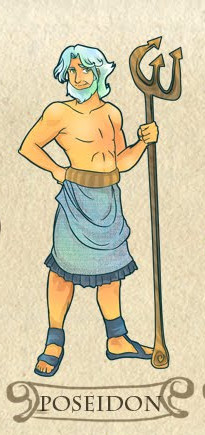
\includegraphics[scale=0.25]{res/characters/poseidom.png}
\caption{Exemplo de poseidom}
\label{poseidom}
\end{figure}

{\large \textbf{Hades}}: sendo um Deus que utiliza maldições para atacar, possuirá dano maior em inimigos do tipo tanker.
\begin{figure}[!htp]
\centering
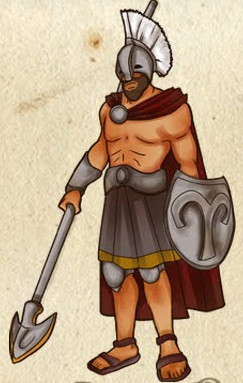
\includegraphics[scale=0.25]{res/characters/hades.png}
\caption{Exemplo de hades}
\label{satiro}
\end{figure}

\subsection{Torres}
Serão duas torres para cada Deus, sendo divididas em dois níveis, para subir de nível e liberar a torre de tier superior é necessário conseguir uma quantia \textit{gold}, hávera também uma torre de tier três, para chegar nesta torre é necessário conseguir acumular uma grande quantia de \textit{gold}. 

\subsection{Waves} 

Haverão diversas \textit{waves}, onde estarão divididas entre 4 categorias, sendo elas normal, tanker, fly e  speed, havendo também um tipo especial de monstro o \textit{Boss}.

\textbf{{ {\large Normal}}} – os inimigos do tipo normal, não terão nenhum beneficio, eles serão \textbf{sátiros}.
\begin{itemize}
\item HP - 50
\item Def - 50
\item Sp -50
\end{itemize}

\begin{figure}[!htp]
\centering
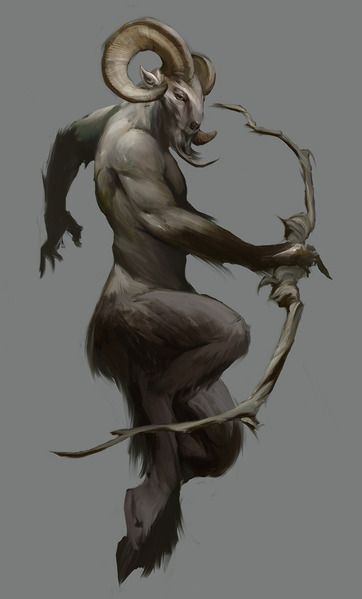
\includegraphics[scale=0.25]{res/characters/satiro.jpg}
\caption{Exemplo de sátiro}
\label{satiro}
\end{figure}

\textbf{{\large Tanker}} – Os \textit{tankers}, serão inimigos que possuirão um HP mais alto do que os outros monstros, sendo necessário vários ataques para causar danos, eles serão os \textit{cyclops}.
\begin{itemize}
\item HP - 150
\item Def - 50
\item Sp - 50
\end{itemize}

\begin{figure}[!htp]
\centering
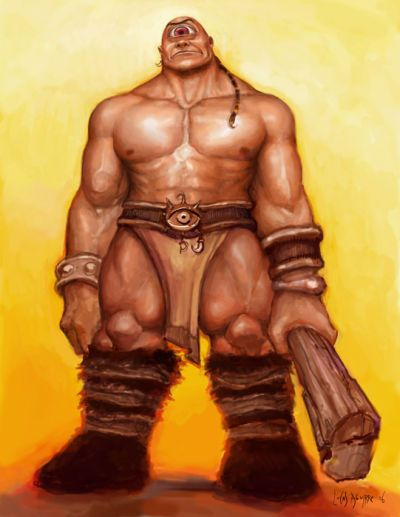
\includegraphics[scale=0.4]{res/characters/cyclops.jpg} \quad
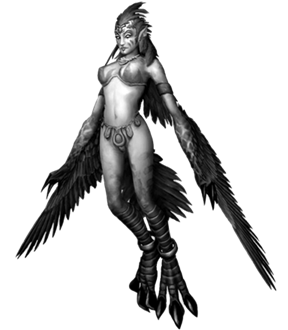
\includegraphics[scale=0.7]{res/characters/harpia.png}
\caption{Exemplo de cyclops e harpia}
\label{cyclops}
\end{figure}

\textbf{{\large Fly}} – Os \textit{Fly}, serão inimigos que possuirão uma defesa elevada sendo necessário ataques fortes para causar dano, porém mantém um hp normal, estes inimigos são as \textit{harpias}.
\begin{itemize}
\item HP - 50
\item Def - 100
\item Sp -50
\end{itemize}

\textbf{{\large Speed}} – Os \textit{Centauros}, serão os inimigos do tipo \textit{speed}, estes possuirão uma alta velocidade, porém um baixo hp.
\begin{itemize}
\item HP - 50
\item Def - 50
\item Sp -80
\end{itemize}

\begin{figure}[!htp]
\centering
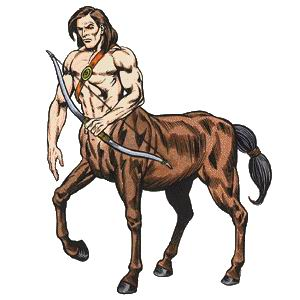
\includegraphics[scale=0.6]{res/characters/centauro.jpg}
\caption{Exemplo de centauros}
\label{cyclops}
\end{figure}

\textbf{{\large Boss}} – Os \textit{Centauros}, o \textit{boss} poderá ser qualquer um dos inimigos anteriores, porém ele irá possuir um tamanho maior do que o de um inimigo comum, além de possuir maior defesa e \textit{HP}.
\begin{itemize}
\item HP - 200
\item Def - 150
\item Sp - 30
\end{itemize}

\newpage

\section{Saúde}

O jogador terá uma barra de vida com 50 HP, a qual decairá a medida que os inimigos atravessem o mapa, sendo que cada tipo de inimigo tem uma pontuação diferente, sendo elas.
\begin{itemize}
 \item Norma = 2 
 \item Tanker = 5
 \item Speed = 3
 \item Fly = 3
 \end{itemize} 

\newpage

\section{Economia}

A única remuneração do jogo será em \textit{gold}, o qual terá como intuito incrementar as torres, não havendo nenhum tempo especifico para a compra de torres, exceto o tempo inicial de jogo, que o jogador seleciona as torres desejadas antes do jogo iniciar de fato, assim as compras podem ser realizadas em qualquer momento da partida.

Os \textit{golds}, são acumulativos ao decorrer das fases, sendo perdidos somente no \textit{game over}.

Toda pontuação do jogador será obtido através dos monstros derrotados, quanto mais forte for o inimigo  maior será a recompensa em ouro, sendo que cada um dos monstros possuem uma pontuação diferente, tal pontuação possui os seguinte valores:

\begin{itemize}
 \item Norma = 2 Golds
 \item Tanker = 5 Golds
 \item Speed = 3 Golds
 \item Fly = 3 Golds
 \end{itemize} 
 
Como as torres tem dois \textit{Tiers}, haverá valores diferentes para as torres de cada \textit{Tiers}, assim para as torres de \textit{Tier 1}, ou seja de nível mais baixo, serão necessários 20 \textit{Golds} para aquisição das mesmas, já para as torres de \textit{Tier 2} será necessária a quantia de 40 \textit{golds} para aquisição das mesmas, caso estas estejam disponíveis, uma vez que para liberar o acesso a torres de \textit{Tier 2} é necessário alcançar 40 golds na torre de \textit{Tier 1} respectiva, por exemplo para liberar as torres de \textit{Tier 2} do \textit{Deus} \textbf{Zeus} é necessário alcançar a marca de 40 golds nas torres de \textit{Tier 1} do \textbf{Zeus}, e assim respectivamente nos outros \textbf{Deuses}.

Não haverá diferenciação nos valores entre as torres por Deuses, somente entre os \textit{Tiers} das torres, assim cada Deus terá torres nos dois \textit{Tiers} existentes.
 
No inicio do jogo, tem-se disponível a quantia de ouro suficiente para a compra de somente duas torres de \textit{Tier 1}, ou seja 40 golds, as quais podem ser de investidas nas torres de qualquer um dos Deuses.  

Caso o jogador se arrependa de ter posicionado uma torre em um local ineficiente, ou por qualquer outro motivo que seja, ele terá a opção de recupera metade do \textit{gold} investido, retirando a torre do local, ou sejá uma torre que custa 20 golds, terá 10 \textit{golds} recuperados.
 
 
O \textit{gold} será representado por um imagem de ouro e uma quantia ao lado da imagem, essa representação será posicionada no canto superior direito da tela. Também tem-se uma imagem contendo o valor de \textit{gold} alcançado por cada torre existente, este valor fica no HUD abaixo da torre em questão.

Resumindo tem-se a seguinte lista com os valores das torres:
\begin{itemize}
 \item Tier 1 = 20 Golds.
 \item Tier 2 = 40 Golds.
 \item Liberar Tier 2 = 40 Golds em uma torre de Tier 1.
 \item Recuperar torre = perca de metade dos golds.
\end{itemize} 

\begin{figure}[!htp]
\centering

\includegraphics[scale=1.25]{res/gold.png}
\caption{Representação Gold}
\label{Tela Equip}
\end{figure}

\begin{figure}[!htp]
\centering

\includegraphics[scale=1.0]{res/torresGold.png}
\caption{Representação Gold associado as torres.}
\label{Tela Equip}
\end{figure}

\section{Esquema de controle e interface com o usuário}

O jogador movimentará somente o mouse, utilizando o mesmo para colocar as torres na posição desejada, sendo que o mesmo seleciona a torre desejada no menu inferior, o mouse indica que a torre foi selecionada, com a torre sobrepondo o cursor do mouse.

Um circulo em volta do cursor será formado, para indicar o alcance de ataque da torre, caso o local para adicionar a torre sejá inválido este circulo ficará avermelhado.  

\newpage

\section{Front End}

O \textit{Front End} do jogo terá  quatro telas principais, sendo elas, menu de \textit{Abertura}, \textit{Fases}, \textit{Gameplay} e \textit{Créditos}, além de uma tela auxiliar de carregamento \textit{loading screen}. A seguir uma representação das telas do jogo.

\subsection{Tela de Abertura}
A tela de abertura do jogo dará acesso para outras duas telas, que são: \textit{Gameplay} e \textit{Credits}.

Nesta tela haverá a imagem do jogo ao fundo, e um menu com as seguintes opções para o jogador: 
\textit{Play Game} que levará o jogador para a tela de \textit{Gameplay}.
\textit{Crédits} para exibição dos créditos.
\textit{Exit} que fechara o jogo.

\begin{figure}[!htp]
\centering
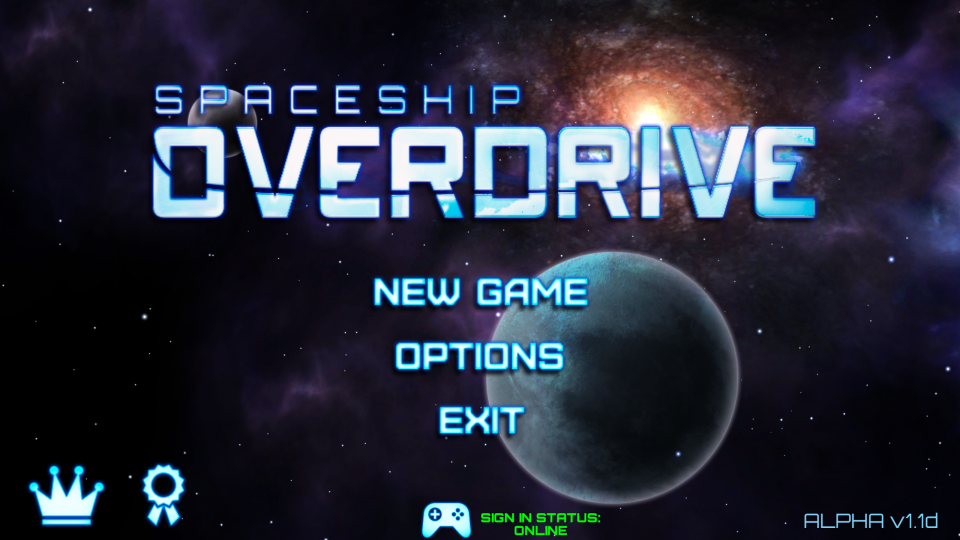
\includegraphics[scale=0.4]{res/abertura.png}
\caption{Exemplo de Abertura}
\label{Abertura}
\end{figure}

\subsection{Tela de Fases}
Nesta tela o jogador escolhe as fases que desejá jogar, ao inicio do jogo somente a primeira fase encontra-se disponível, para abrir as subsequentes é necessário sobreviver nas fases anteriores.

As fases abertas estarão com uma imagem do mapa visível, já as imagens fechadas estarão cinzas.

Nesta tela, haverá também um ícone para voltar a tela anterior.  

Ao selecionar uma fase, aparecerá uma mensagem pedindo a confirmação da escolha e o jogador será redirecionado para a página de \textit{Gameplay}, caso concorde.

\begin{figure}[!htp]
\centering
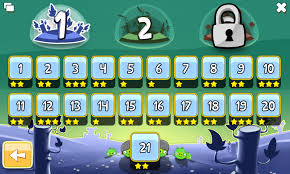
\includegraphics[scale=1]{res/fases.jpg}
\caption{Exemplo da tela de fases}
\label{Fases}
\end{figure}

\newpage

\subsection{Tela de Gameplay}

Tela principal do jogo, nesta tela tem-se um menu na parte inferior da tela, com as informações do Deus no quadro inferior esquerdo, ao clicar no Deus sua torre é selecionada e aparece no quadro inferior direito.
No quadro inferior central tem-se as informações sobre as torres, sendo que as torres disponíveis ficam com a imagem da torre visível já as torres indisponíveis ficam com um "\textbf{x}", há também um pequeno quadro indicando quanto de \textit{gold} falta para evoluir a torre e liberar o próximo tier.

Para adicionar uma nova torre o jogador deverá clicar na torre no box inferior direito e arrasta-lá no mapa até a posição desejado.

O mapa fica no centro da tela, ocupando o máximo de área possível.

Na parte superior direita haverá um relógio contendo o tempo restante de fase.

Na parte superior central tem-se informações sobre as \textit{waves}.

\begin{figure}[!htp]
\centering
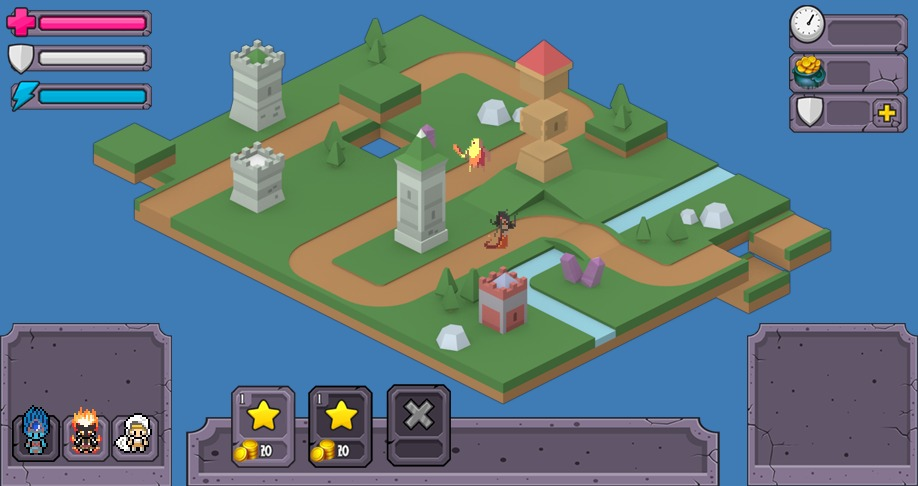
\includegraphics[scale=0.5]{res/gameplay.jpg}
\caption{Exemplo de Gameplay}
\end{figure}

\newpage
\subsection{Tela de Créditos}

Na tela de \textit{Cr} exibe-se o nome e a função de cada um dos integrantes da equipe, sendo de \textit{Desnvolvimento}, \textit{artes} e \textit{música}.

\newpage

\subsection{Logo}

A logo a seguir o logo do SomTD].
\begin{figure}[!htp]
\centering

\includegraphics[scale=1.1]{res/logo.png}
\caption{Logo do SomTD}
\label{Logo do SomTD}
\end{figure}

A logo a seguinte representa a API utilizada durante o desenvolvimento.

\begin{figure}[!htp]
\centering

\includegraphics[scale=0.3]{res/Sdl-logo.png}
\caption{Logo da SDL}
\label{Logo da SDL}
\end{figure}

\begin{figure}[!htp]
\centering

\includegraphics[scale=0.3]{res/classification.png}
\caption{Classificação Indicativa}
\label{Classificação Indicativa}
\end{figure}

A classificação indicativa definida foi de 12 anos, devido a possíveis traços de violência no jogo, . 


\newpage

\section{Requisitos tecnológicos}

\begin{figure}[!htp]
\begin{center}
  
\includegraphics[scale=0.04]{res/audacity.png} \quad
  
\includegraphics[scale=0.3]{res/adobe_illustrator.png} \quad
  
\includegraphics[scale=0.25]{res/Sdl-logo.png} \quad
  
\includegraphics[scale=0.3]{res/Sublime_Text_Logo.png} \quad
  
\includegraphics[scale=0.2]{res/cpp.png} \quad
  
\includegraphics[scale=0.13]{res/git.png} \quad
  
\includegraphics[scale=0.5]{res/linux.png} \quad
\caption{Recursos Tecnológicos} \label{gdimotes}
\end{center}
\end{figure}

\section*{Informações de contato}
{\Huge \textbf{strifeofmythology@gmail.com}}

\end{document}
